
\documentclass[a4paper]{article}
\usepackage{amsfonts}
\usepackage{amsmath}
\usepackage{amssymb}
\usepackage{graphicx}     
\newcommand{\ddx}{\dfrac{d}{dx}}
\newcommand{\ddg}{\dfrac{d}{dg}}
\newcommand{\limy}{\displaystyle\int\limits_0^{2\pi}}
\begin{document}
  
\noindent \large Auteur: Luca Letroye \\
\noindent \large Studierichting: Informatica\\
\noindent \large Oefeningenreeks 5K nr. 1.3.\

\medskip

\normalsize

$r = 2-2\cos\theta$\\

$r' = 2\sin\theta$

$ L = \limy \sqrt{(2-2\cos(\theta))^2 +(2\sin(\theta)^2)}d\theta $\\

$ =  \limy \sqrt{4(1-\cos(\theta))^2 +4\sin(\theta)^2}d\theta $\\

$  = \limy 2\sqrt{(1-\cos(\theta))^2 +\sin(\theta)^2}d\theta $\\

$ =  \limy 2\sqrt{1- 2\cos(\theta) + \cos^2(\theta) +\sin^2(\theta)}d\theta $\\

$ = \limy 2\sqrt{2- 2\cos(\theta)}d\theta $\\

$ = \limy 2 \cdot \sqrt{2} \cdot \sqrt{2} \sin{\dfrac{\theta}{2}} d\theta $\\

$ =  \limy  4\sin{\dfrac{\theta}{2}} d\theta $\\

$ =  8[-\cos(u)]_0^{\pi} $\\

$ =  16 $\\

\begin{figure}[h]
\centering
	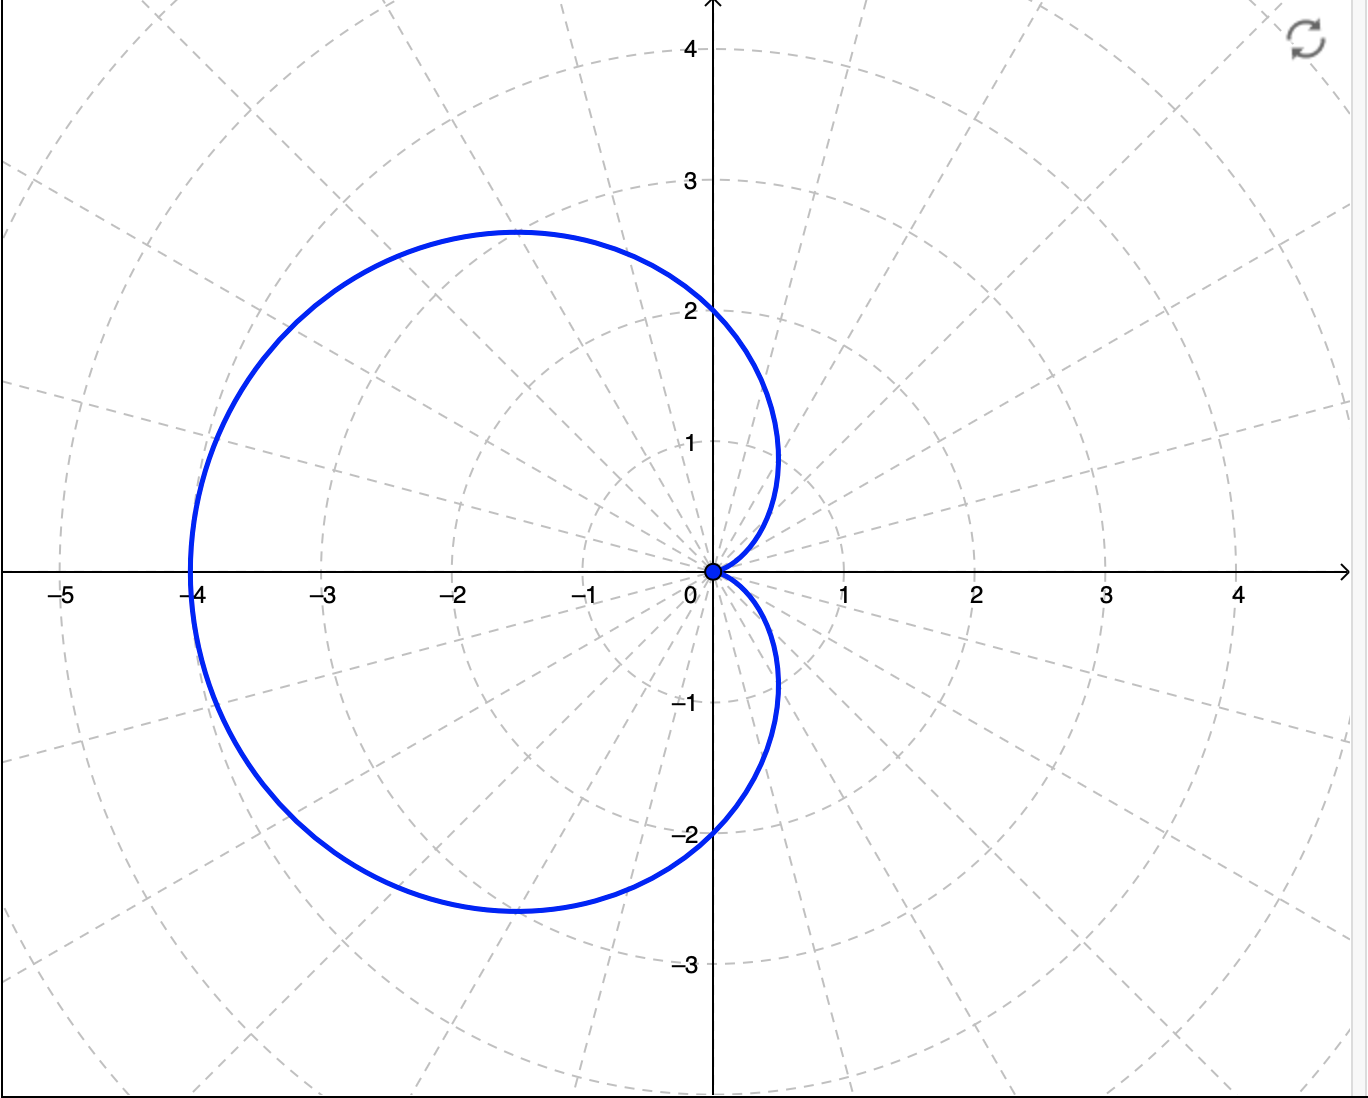
\includegraphics[width=6cm]{5K-1.3-luca.letroye.INF.png}
\end{figure}



\begin{thebibliography}{999}
%\bibitem{a} Referentie
\end{thebibliography}

\end{document}
